
\documentclass[a4paper]{report}
\newtheorem{mydef}{Definition}
\usepackage{graphicx}

\begin{document}

\title{Study On NP-complete problems}
\author{Adam Jama}
\date{February 2013}

\maketitle

\pagenumbering{roman}

\chapter{Definition Of 8 Problems}

\subsection{Graph Colouring}
\begin{mydef}
adam In graph computational theory the graph colouring problem is a special assignment of which is traditionally assigned with colours. In the more common approach of the graph colouring problem is a way of colouring the vertices of an undirected graph such that no two adjacent vertices share the same colour.
\end{mydef}

There are three fundamental steps with the graph colouring process. The first is the decision process which we input a graph $\emph{G}$ with $\emph{n}$ vertices and choose an integer $\emph{K}$ where the graph colouring problem decision in yes. The example of the first case where the decision would be NP-complete would be the 3 colouring as shown below.



\begin{center}
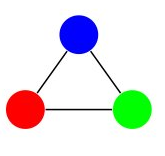
\includegraphics[scale=0.77]{3colouring.png}
\end{center}

The output of the decision would be whether or not the graph $\emph{G}$ admits a proper vertex colouring with $\emph{k}$ colours. There is also a special case where a graph is 2 colourable and can be be done in $\emph{P}$ (Polynomial-time) and this is were the particular graph that we're colouring is bipartite which is a particular graph whose vertices can be divided into two disjoint sets were every edge that connects a vertex in $\emph{U}$ to one in $\emph{V}$.



\vspace{3mm}
The next step with graph colouring would be the optimisation which the chromatic number. The chromatic number refers to the smallest number of colours needed to colour a graph $\emph{G}$ is called the chromatic number and is often denoted by $\emph{X}$($\emph{G}$). With the optimisation process we will have an input of a graph $\emph{G}$ with $\emph{n}$ vertices. We will firstly have a look at the simplest form which is not bipartite. We have looked at this previously which is the triangle $\emph{K}$$^{3}$.

\vspace{3mm}
The first example that I will show is that a complete graph $\emph{K}$$^{3}$ with $\emph{n}$ vertices is $\emph{n}$-colourable but not (n-1) colourable. This is shown below showing that $\emph{K}$$^{3}$ is not 2 colourable. Another rule we would have to follow would be that $\emph{K}$$_{n}$ has a vertex set $\lbrace$1,...,n$\rbrace$ and all possible $\frac{1}{2}$ $\emph{n}$ ($\emph{n}$-1) edges. I will look at another example to prove the chromatic number which will be the graph $\emph{K}$$_{4}$ with 4 vertices is 4 colourable as shown below:



\end{document}